
%\renewcommand{\familydefault}{\sfdefault}
%=============== En−Tete ===============
 
%−−− Insertion de paquetages −−−−
\documentclass[12pt,a4paper]{report}
\usepackage[utf8]{inputenc}
\usepackage{amsmath}
\usepackage{amsfonts}
\usepackage{amssymb}
\usepackage{graphicx}
\usepackage{wrapfig}
\graphicspath{ {./images/} }
\usepackage[rightcaption]{sidecap}
\usepackage{subcaption}

\usepackage[french]{babel}
\usepackage[Bjarne]{fncychap}
\usepackage{fancyhdr}
\usepackage{float}
\usepackage{epsfig}
\usepackage{appendix}
\usepackage[final]{pdfpages}
\usepackage{array}
\usepackage{pdfpages}

\pagestyle{fancy}


\usepackage{titlesec}
%-\titleformat{\chapter}[display]{\bfseries}{\huge\chaptertitlename~\thechapter}{10pt}{\LARGE}--%

%−−− Page de garde - titre −−−

\begin{document}

\title{\Large{\Large {Travail de lecture et de rédaction scientifique sur le Federate Learning}}}

\author{Bal Sébastien}

\maketitle

\thispagestyle{empty} % Ignore page number

\fancyhead[LE,RO]{\leftmark}

\fancyhead[RE,LO]{}



 

%=============== Remerciement ===============

\begin{figure}[p]

\large\textbf{Remerciements}


\end{figure}

\tableofcontents
\thispagestyle{empty} % Ignore page number

\fancyfoot[C]{Master en Science infomatique - Lecture et rédaction scientifique}
\fancyfoot[R]{\thepage}

\chapter{Machine Learning}
\thispagestyle{plain}\setcounter{page}{1} % Start page count
Le Machine Learning appelé en Français apprentissage automatique [x: wikipédiea] a pour objectif de traiter l'information afin de lui donner de la valeur ajoutée.\\

De nos jours, le Machine Learning est présent partout sur la toile, cela va du moteur de recherche comme Google, aux assistants vocaux comme Siri et Alexa, les fil d'actualités des réseaux sociaux comme Facebook et Twitter. Le point commun entre toutes ces platformes et le stockage massif des données de leur utilisateur appelé Big Data [x: ?]. Le Big Data est une technologie apparue dans les années xxxx, a permis l'essor de l'apprentissage automatique, le Machine Learning. En effet, cet imposant volume de données collectées sur les utilisateurs a permis, dans les exemples cités ci dessus, de mieux cibler le comportement des utilisateurs et donc améliorer les expériences.\\

Pour fonctionner, le Machine Learning(ML) a besoin de données à ingérer et d'avoir un modèle appris afin de fournir des données à valeur ajoutée comme des algorithmes de prédiction de bourse et la maintenance prédictive. Il est donc nécessaire d'identifier les solutions pour créer ces modèles de ML.\\

\begin{center}
	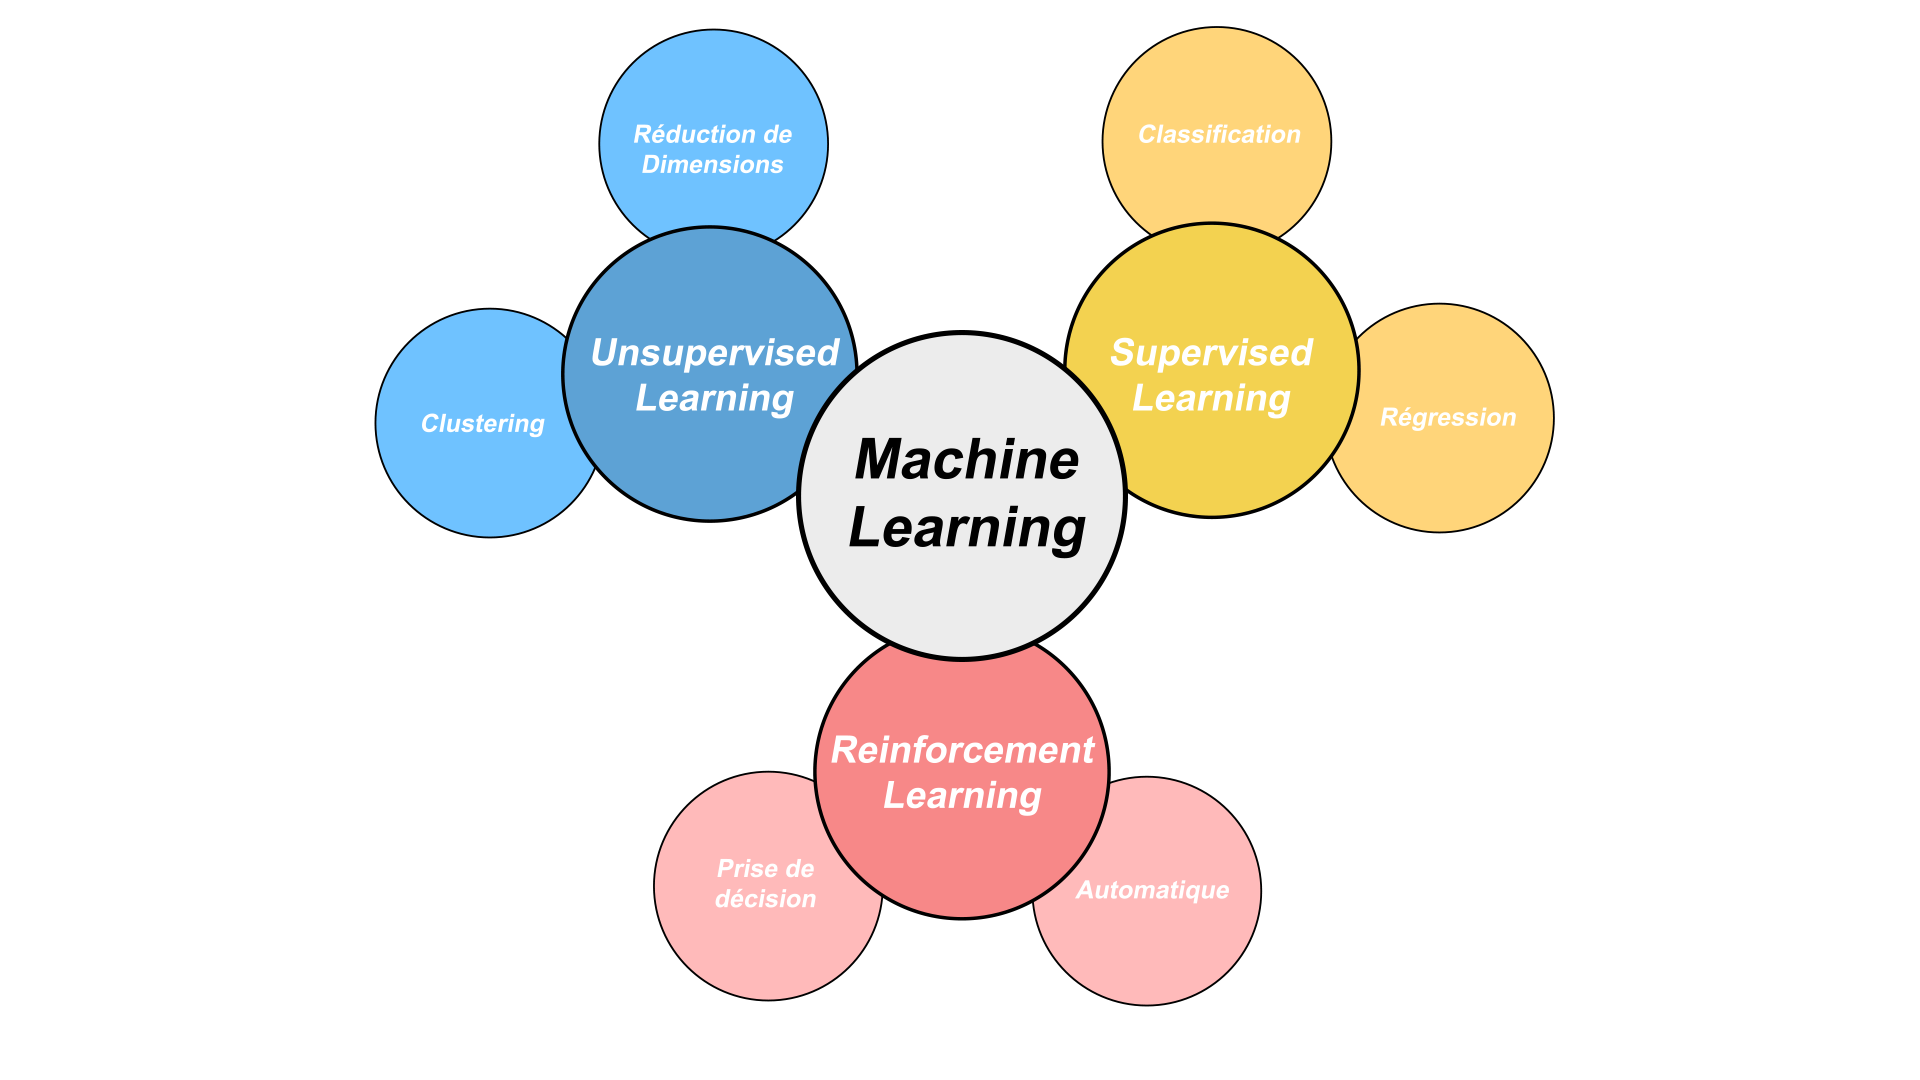
\includegraphics[scale=0.2]{ML_vignette}
	\captionof{figure}{Familles d'algorithmes les plus utilisés}
	\label{fig1}
\end{center}

La première famille, l'appentrissage supervisé (en jaune dans la figure 1.1) consiste à donner des données en entrées, le résultat attendu itéré sur un grand jeu de données afin de trouver la modèle. Pour que le modèle deviennent performant, on fournit un grand volume de données dans le but qu'il se rapproche du modèle attendu.\\

La deuxième famille,l'apprentissage non-surpervisé (en bleu dans la figure 1.1) consiste à apprendre par reconnaitre des ressemblances et des différences entre les données fournies. L'algorithme rassemble les données en groupe suivant ce qui lui semble le plus pertinant. Ainsi quand on passe un modèle bien précis à l'algorithme, il trouve plus facilement car il a été entrainé.\\

Pour finir, il existe une catégorie qui gère sa propre expérience. En effet, l'apprentissage par renforcement (en rouge dans la figure 1.1) consiste à générer ses propres expériences. On se rapproche de l'automobile autonome, la machine change ses états suivant les actions qu'elle entreprend de faire. Un système de récompense positive et négative est mis en place pour constituer une nouvelle expérience et rendre la machine attentive pour maximiser ses chances de réussite.\\
\pagebreak

Pour conclure, le ML est une technologie qui vise à trouver des modèles, comprendre des comportements afin de prédire les besoins d'une application suivant un utilisateur.\\

On peu constater que ce type de besoin se focalise sur une application spécifique cependant, le ML connait des limites au niveau des complexités combinatoire [x: ], or certaines applications nécessitent des applications plus complexes avec plus d'entrées, tels que le traitement des images. Pour palier aux limites du ML, le Deep Learning a vu son essort [x: lien vers essort DL]
\pagebreak



\chapter{Deep Learning}
\section{Les concepts}

Le Deep Learning(DL) est représentatif d'un système neuronal comme notre système cérébral, il est conçus de plusieurs neuronnes qui intéragissent entre eux. Pour rendre performant tous ces neuronnes, il est nécessaire d'avoir une grande quantité de données, un Data Lake. Celui ci fournit au système plusieurs informations afin de lui constituer une "mémoire". Cette mémoire lui permet de reconnaitre des éléments bien particulier suivant l'entrainement qu'il aura suivit. Cet entrainement est supervisé par des développeurs qui vérifient que le DL ne sort pas de son modèles définis.
Si il s'en éloigne, ils corrigent son algorithme mathématique pour le rendre performant et le remettre sur le droit chemin. Pour que le modèle mathématique deviennent performant, il faudra l'entrainer à reconnaitre une donnée en particulier. C'est le sujet de notre prochaine section.


\pagebreak

\section{Modèle d'entraînement}

Pour entrainer le DL, il lui faut un algorithme mathématique et un grand flux de données afin d'affiner ses recherches et prendre de l'expérience. Dans notre situation, on décider de prendre la reconnaissance d'une image, en particulier celle d'un chat.
On fournit à l'algorithme un flux d'images de plusieurs espèces d'animaux, on définit les paramètres qui permettent d'affirmer que l'image que l'on soumet soit bien un chat. Ainsi avec ces critères, l'algorithme devient plus précis car on le guide un peu sur l'objectif qu'il doit atteindre.
 
Voici un schéma pour l'exemple du fonctionnement du DL,[fig2.1], les boules vertes représente le bon chemin que le système va prendre pour arriver à vérifier le modèle qui était demandé. Les boules bleus sont celles qui ont des caractéristiques avec le modèle mais ne correspondra pas exactement au modèle qui était demandé. Les boules rouges quand à elles, représentent les erreurs que le système a exclu pour pouvoir apprendre le modèle exacte. Les erreurs sont par la suite renvoyées en amont du système pour que le système ajuste son modèle mathématique

\begin{center}
	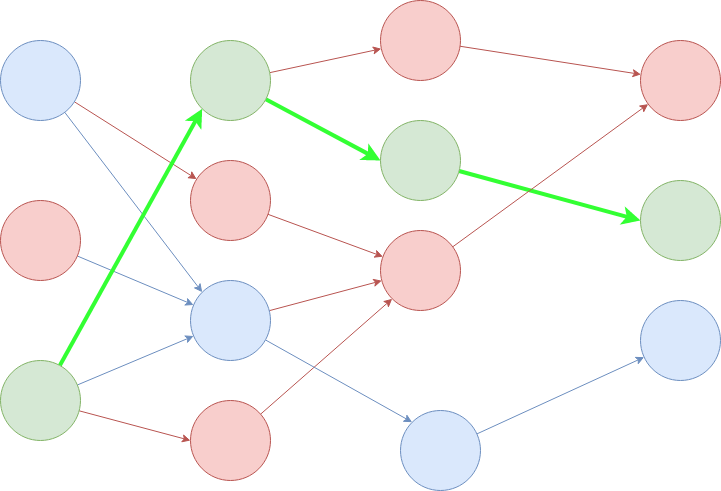
\includegraphics[scale=0.4]{deep_learning_schema}
	\captionof{figure}{Autoapprentissage Deep Learning}
	\label{fig1}
\end{center}

On peut constater que ce type d'algorithme peut être très vite devenir énergivore. De plus, le DL se focalise principalement sur une application. Or, il peut être intéressant d'étudier plusieurs applications similaires afin d'identifier des modèles plus poussés. C'est dans ce contexte que nous allons introduire le Federated Learning.


\chapter{Federated Learning}
\section{Définition du Federated Learning}


Notre époque fait face à deux défis importants en terme d'avencer technologique: les respects des données des utilisateurs et l'augmentation du volume des données.

L'une des plus importantes est celle de la privatisation de ces données sur le web. Avec la protection des données (RGPD) promulgué en 2018, les données privées font entièrement partie de l'utilisateur. Ces données ne peuvent pas être utilisé sans son accord.

Ensuite le silo des données met un frein à l'évolution de l'industrie moderne, c'est en ayant plus de données que l'on peut améliorer la qualité de la formation. Cependant le manque de données valides dans le domaine médical vient principalement du faite que les travailleurs doivent être expérimentés dans certains domaines comme celui de l'industrie médicale.

C'est grâce au Federated Learning(FL) que l'essort de l'industrie a relevé ces défis. Car le FL est un processus d'apprentissage automatique qui vise a exploité les îlots de données tout en gardant la sécurité des données.




En quelques mots, c'est un apprentissage automatique distribué qui permet d'entraîner un modèle mathématique avec un large groupe de données décentralisées qui se trouvent sur des téléphones portables(pour notre cas ici).



\section{Implémentation}
Dans notre modèle, nous allons utilisé le système TensorFlow pour former notre système neuronal. TensorFlow est une bibliothèque open source pour le Machine Learning. C'est un petit couteau Suisse qui contient ici des outils pour permettre de résoudre des problèmes mathématiques. 

\section{Deep Learning, cas d'utilisation}

\subsection{Smart Building}

\subsection{Industrie}




\begin{thebibliography}{9}

	\bibitem{lamport94}
	  Leslie Lamport,
	  \emph{\LaTeX: A Document Preparation System}.
	  Addison Wesley, Massachusetts,
	  2nd Edition,
	  1994.
	  
	\bibitem{bigdata}
	Pour la partie sur le Machine Learning https://www.lebigdata.fr/machine-learning-et-big-data

\end{thebibliography}


\label{Pour la partie sur le Machine Learning https://www.lebigdata.fr/machine-learning-et-big-data}

\label{TensorFlow : https://www.lebigdata.fr/tensorflow-definition-tout-savoir}

%Citeseer citeseer.ist.psu.edu,Google Scholar scholar.google.com,ScienceDirect www.sciencedirect.com,ACM Digital Library portal.acm.org,IEEE Digital Library www.computer.org/portal/site/csdl/index.jsp


\label{https://www.youtube.com/watch?v=QR1SnCRungE&ab_channel=AlainOlivetti} 


\begin{appendix}
 \chapter{Annexe}
 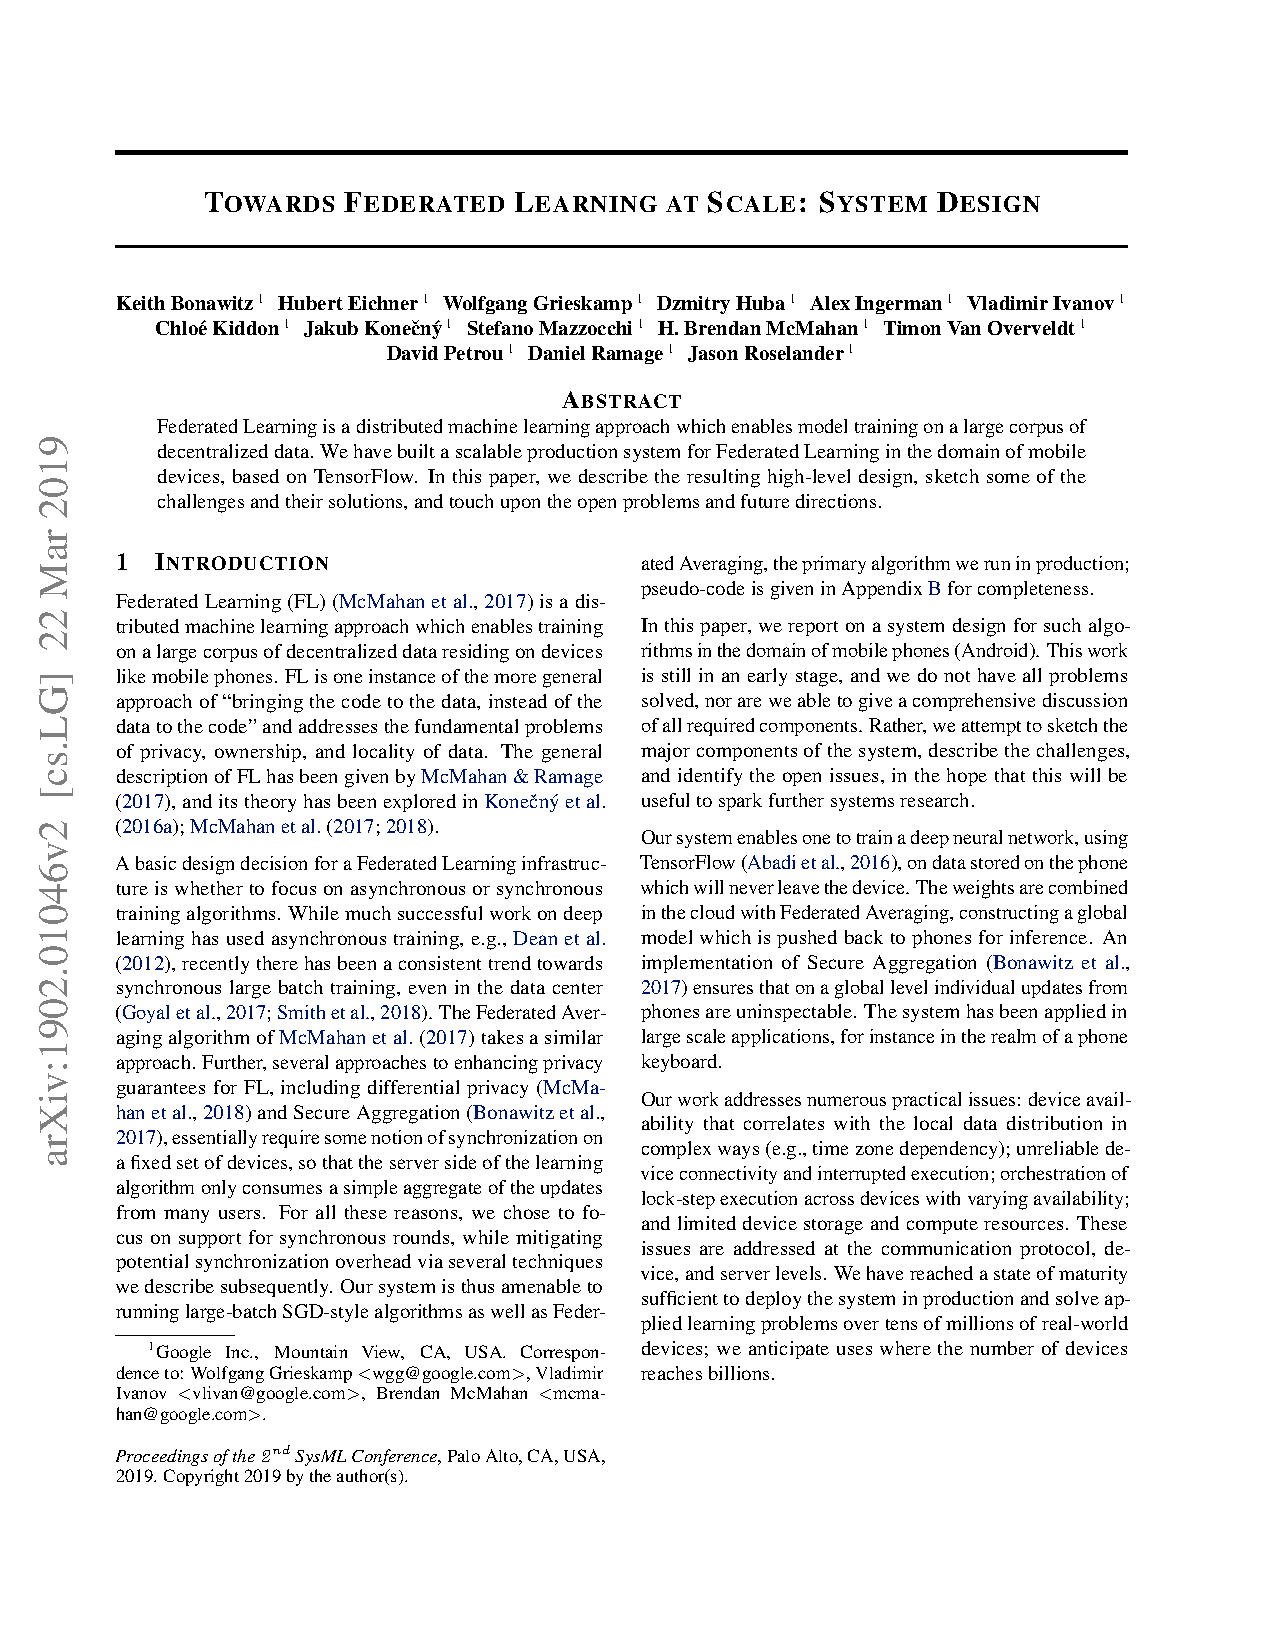
\includepdf{pdf/federate_learning_en.pdf}
\end{appendix}

\end{document}
